\chapter{APPENDIX \label{ch:appendix}}

\section{Final coefficients \label{sec:app:final_coefficients}}
\begin{table}
    \centering
    \begin{tabular}{c|c|c|c}
         \thead{Coefficient} & \thead{Phase II} & \thead{Phase III} & \thead{Phases II + III} \\ \hline
         \makecell{$a^B$} & \makecell{1.02394} & \makecell{1.00341} & \makecell{1.03179} \\
         \makecell{$b^B$} & \makecell{1.08484} & \makecell{1.06898} & \makecell{1.07573} \\
         \makecell{$c^B$} & \makecell{1.18253} & \makecell{1.12627} & \makecell{1.16176} \\
         \makecell{$x_0^B$} & \makecell{0.0344209} & \makecell{0.0131758} & \makecell{0.0269842} \\
         \makecell{$y_0^B$} & \makecell{-0.22116} & \makecell{-0.212521} & \makecell{-0.219484} \\
         \makecell{$z_0^B$} & \makecell{-0.195463} & \makecell{-0.192554} & \makecell{-0.195859} \\
         \hline
         \makecell{$a^g$} & \makecell{0.969417} & \makecell{0.978286} & \makecell{0.97323} \\
         \makecell{$b^g$} & \makecell{0.959791} & \makecell{0.948732} & \makecell{0.957992} \\
         \makecell{$c^g$} & \makecell{0.964618} & \makecell{0.926156} & \makecell{0.953446} \\
         \makecell{$x_0^g$} & \makecell{-0.00218403} & \makecell{0.00733717} & \makecell{0.00149607} \\
         \makecell{$y_0^g$} & \makecell{-0.0149083} & \makecell{-0.0113024} & \makecell{-0.014287} \\
         \makecell{$z_0^g$} & \makecell{0.0218019} & \makecell{0.0260466} & \makecell{0.0251443} \\
    \end{tabular}
    \caption{Coefficents determined from measurement on 11 April 2025.}
    \label{tab:app:coeff}
\end{table}

\begin{table}
    \centering
    \begin{tabular}{c|c|c|c|c|c|c}
             &   xa0  &   ya0  &   za0  &   aa   &   ba   & ca \\
         xa0 &  1     &        &        &        &        &    \\
         ya0 & -0.005 &  1     &        &        &        &    \\
         za0 &  0.016 &  0.007 &  1     &        &        &    \\
         aa  &  0.522 & -0.000 &  0.005 &  1     &        &    \\
         ba  &  0.010 &  0.251 &  0.011 &  0.003 &  1     &    \\
         ca  & -0.008 & -0.015 & -0.273 & -0.007 & -0.013 &  1 \\
    \end{tabular}
    \caption{Correlation matrix of Phase II Acc}
\end{table}

\begin{table}
    \centering
    \begin{tabular}{c|c|c|c|c|c|c}
             &   xm0  & ym0    &   zm0  &   am   &   bm   & cm \\
         xm0 &  1     &        &        &        &        &    \\
         ym0 &  0.096 &  1     &        &        &        &    \\
         zm0 &  0.114 &  0.013 &  1     &        &        &    \\
         am  & -0.457 & -0.055 & -0.105 &  1     &        &    \\
         bm  &  0.180 & -0.212 & -0.045 & -0.212 &  1     &    \\
         cm  &  0.229 &  0.065 &  0.282 & -0.252 & -0.093 & 1  \\
    \end{tabular}
    \caption{Correlation matrix of Phase II Mag}
\end{table}

\begin{table}
    \centering
    \begin{tabular}{c|c|c|c|c|c|c}
             &   xa0  &   ya0  &   za0  &   aa   &   ba   & ca \\
         xa0 &  1     &        &        &        &        &    \\
         ya0 &  0.030 &  1     &        &        &        &    \\
         za0 &  0.093 &  0.017 &  1     &        &        &    \\
         aa  & -0.246 & -0.004 &  0.047 &  1     &        &    \\
         ba  & -0.021 & -0.034 & -0.055 & -0.229 &  1     &    \\
         ca  & -0.017 &  0.053 &  0.280 & -0.098 & -0.195 &  1 \\
    \end{tabular}
    \caption{Correlation matrix of Phase III Acc}
    \label{tab:my_label}
\end{table}

\begin{table}
    \centering
    \begin{tabular}{c|c|c|c|c|c|c}
             &   xm0  & ym0    &   zm0  &   am   &   bm   & cm \\
         xm0 &  1     &        &        &        &        &    \\
         ym0 &  0.053 &  1     &        &        &        &    \\
         zm0 &  0.006 &  0.009 &  1     &        &        &    \\
         am  &  0.266 &  0.015 & -0.033 &  1     &        &    \\
         bm  & -0.013 & -0.073 &  0.014 & -0.234 &  1     &    \\
         cm  & -0.017 & -0.046 & -0.222 & -0.185 & -0.203 & 1  \\
    \end{tabular}
    \caption{Correlation matrix of Phase III Mag}
\end{table}

\begin{table}
    \centering
    \begin{tabular}{c|c|c|c|c|c|c}
             &   xa0  &   ya0  &   za0  &   aa   &   ba   & ca \\
         xa0 &  1     &        &        &        &        &    \\
         ya0 & -0.001 &  1     &        &        &        &    \\
         za0 &  0.067 &  0.004 &  1     &        &        &    \\
         aa  &  0.283 & -0.008 &  0.049 &  1     &        &    \\
         ba  & -0.029 &  0.206 &  0.012 & -0.058 &  1     &    \\
         ca  & -0.053 & -0.008 & -0.127 & -0.065 & -0.046 &  1 \\
    \end{tabular}
    \caption{Correlation matrix of Phases II+III Acc}
\end{table}

\begin{table}
    \centering
    \begin{tabular}{c|c|c|c|c|c|c}
             &   xm0  & ym0    &   zm0  &   am   &   bm   & cm \\
         xm0 &  1     &        &        &        &        &    \\
         ym0 &  0.074 &  1     &        &        &        &    \\
         zm0 &  0.057 &  0.002 &  1     &        &        &    \\
         am  & -0.229 & -0.022 & -0.070 &  1     &        &    \\
         bm  &  0.135 & -0.190 & -0.039 & -0.199 &  1     &    \\
         cm  &  0.142 &  0.038 &  0.134 & -0.215 & -0.121 & 1  \\
    \end{tabular}
    \caption{Correlation matrix of Phases II+III Mag}
\end{table}

\begin{figure}
    \centering
    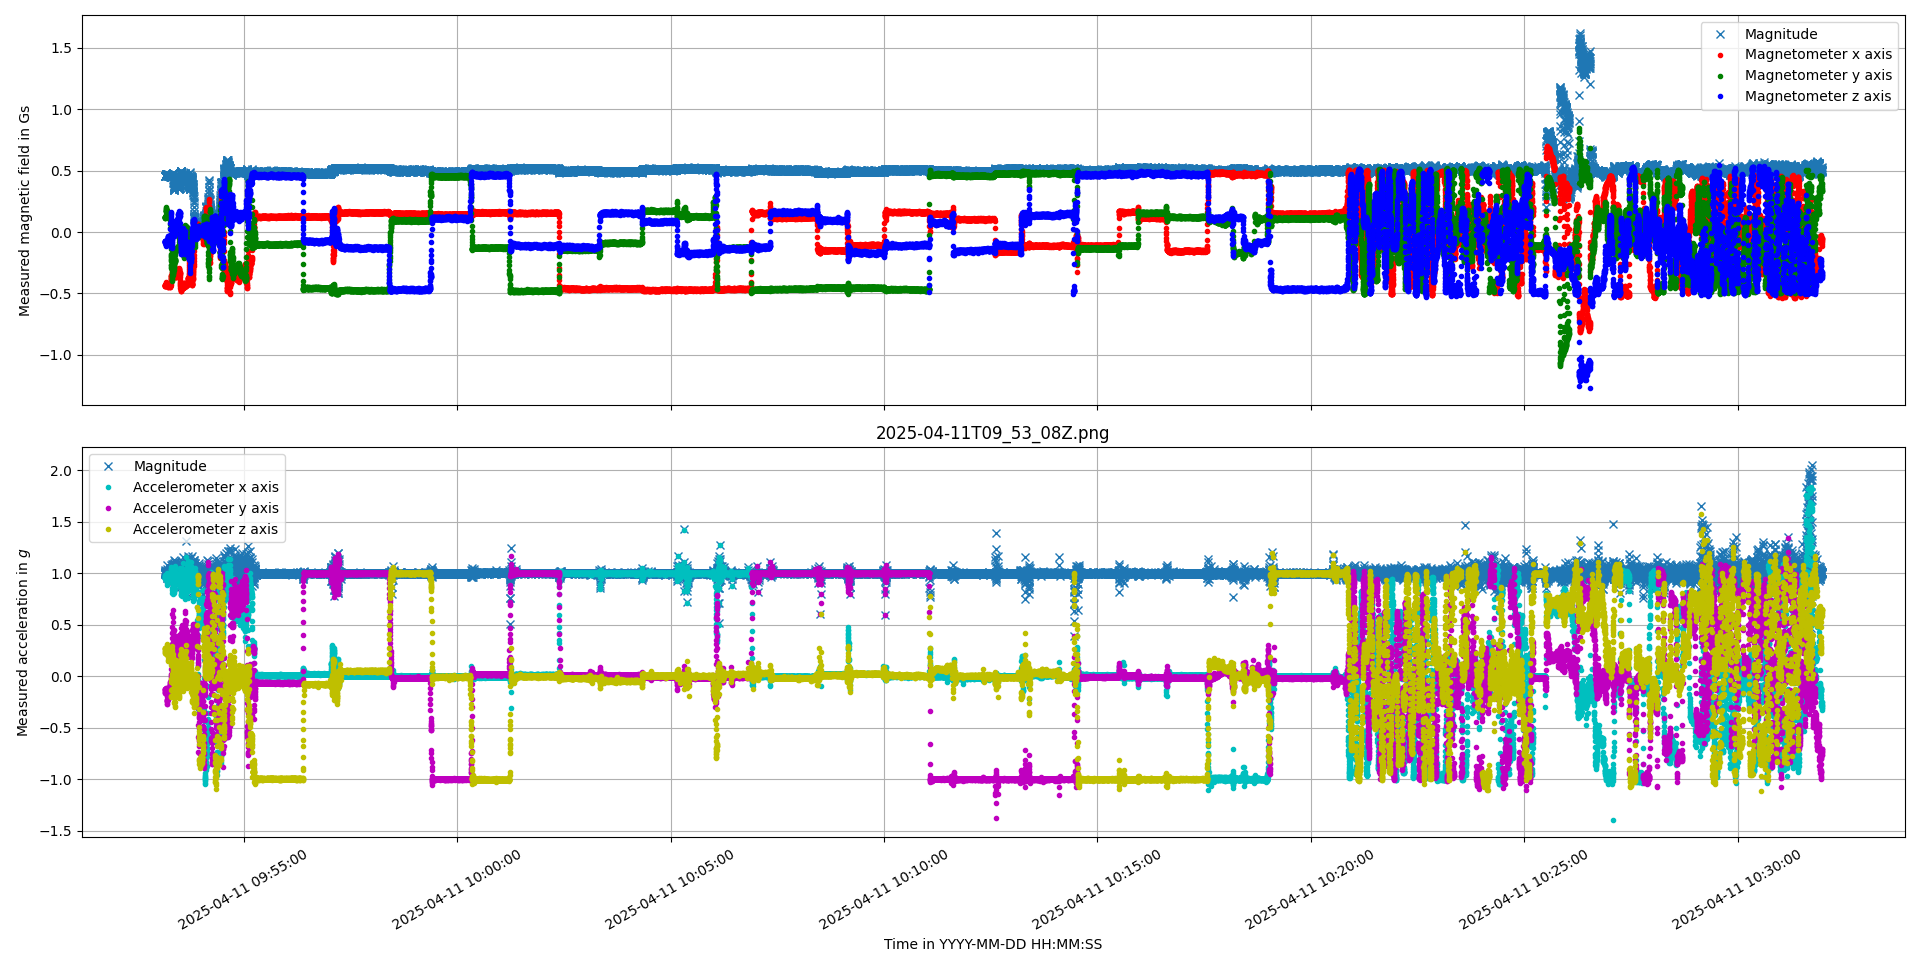
\includegraphics[width=\linewidth]{images/04_results/phaseii_calibrated_calibration11apr.png}
    \caption{Calibrated using coefficients from Phase II}
\end{figure}

\begin{figure}
    \centering
    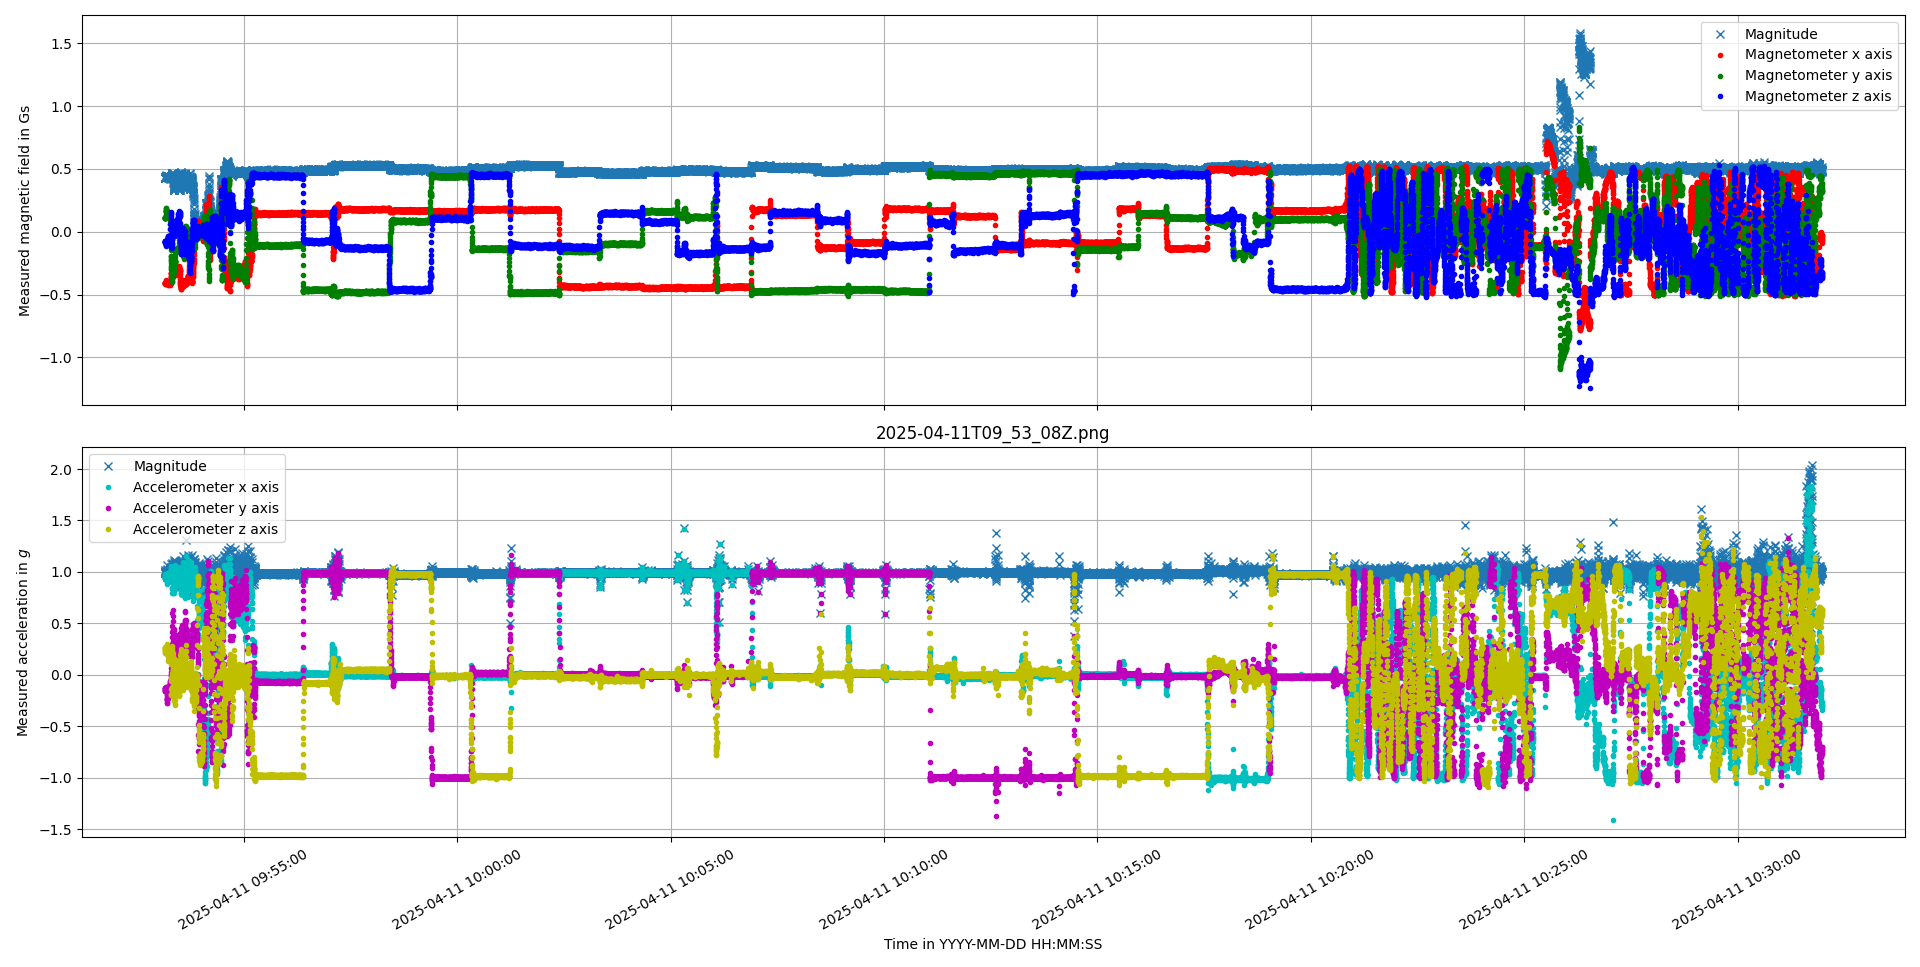
\includegraphics[width=\linewidth]{images/04_results/phaseiii_calibrated_calibration11apr.png}
    \caption{Calibrated using coefficients from Phase III}
\end{figure}

\begin{figure}
    \centering
    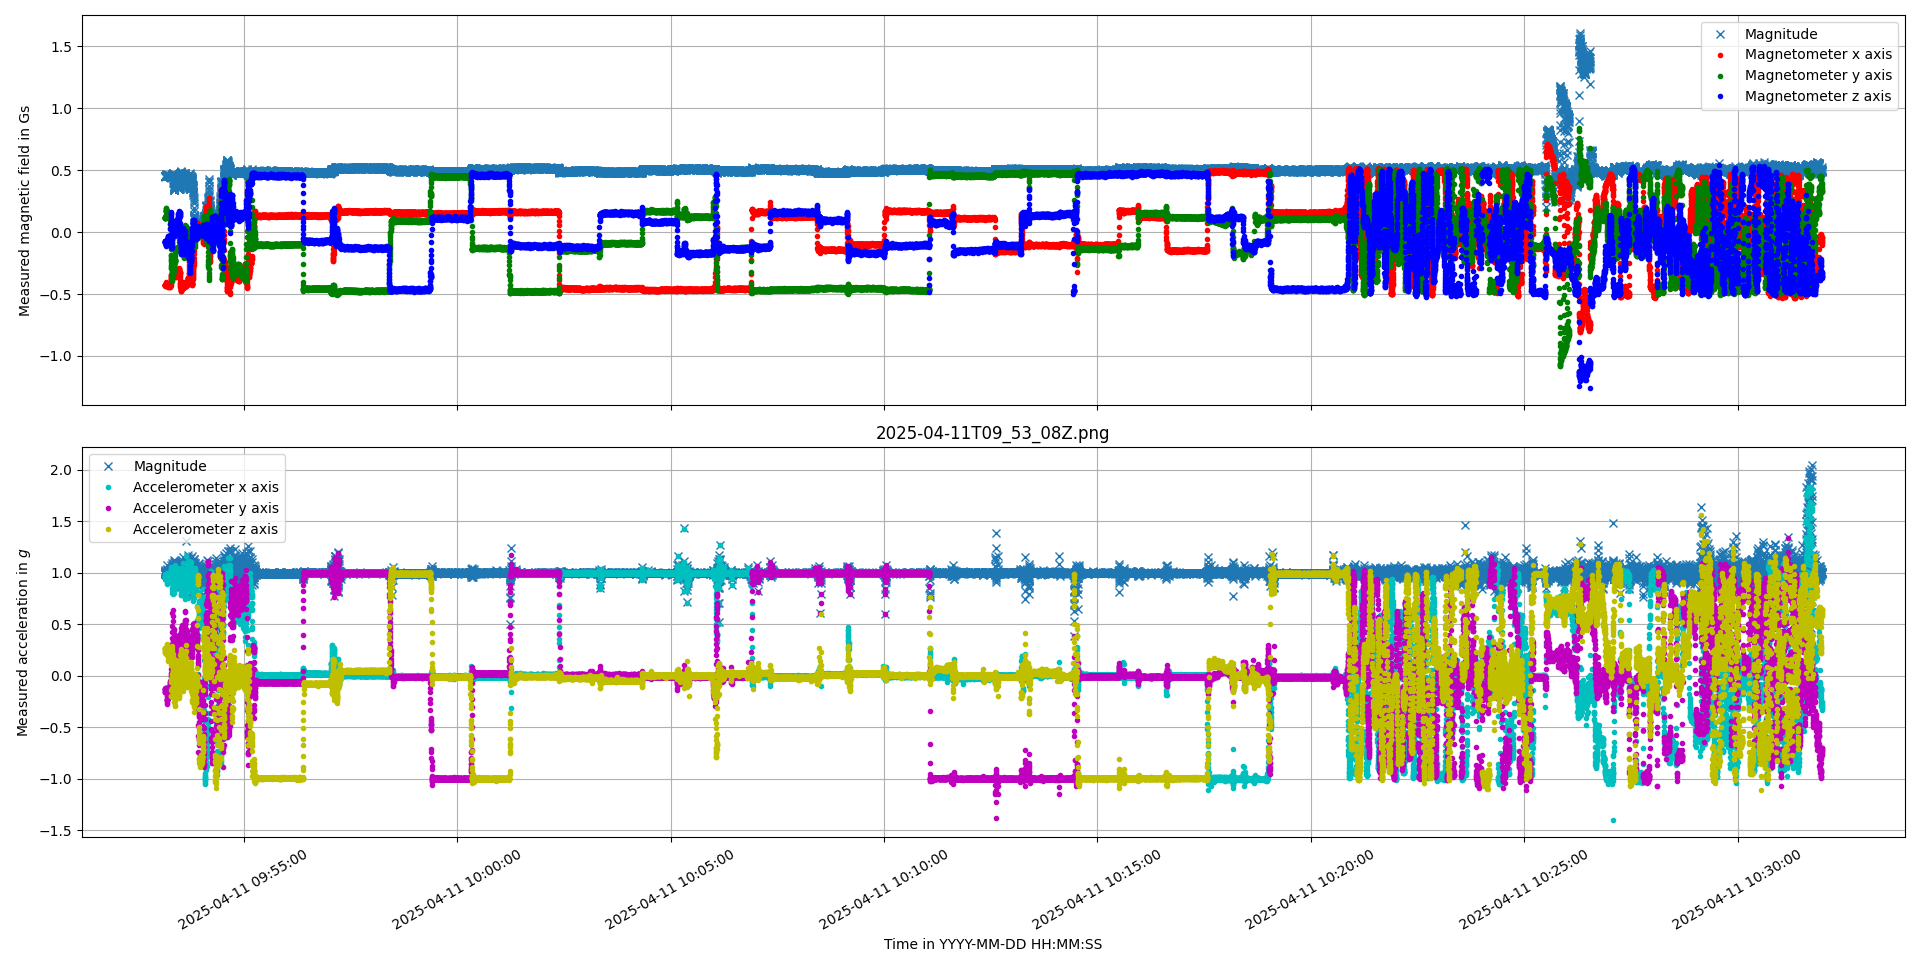
\includegraphics[width=\linewidth]{images/04_results/phaseii_and_iii_calibrated_calibration11apr.png}
    \caption{Calibrated using coefficients from Phases II and III}
\end{figure}


\section{Derivation of Coefficients \label{sec:app:deriv_of_coeff}}
The vector of the measured magnetic field is:
\begin{equation}
    B_{meas}=
\end{equation}


The (magnetic) vector field to be measured is:
\begin{equation}
    B_H=\begin{pmatrix} B_x \\ B_y \\ B_z \end{pmatrix}
\end{equation}

Assume the z-axis as fixed or true, then the measured value (denoted by the hat) is the true value $B_z$ scaled by $c$ and offset by $z_0$:
\begin{align}
    \hat{B}_z&=cB_z+z_0 \\
    \iff B_z&=\frac{\hat{B}_z-z_0}{c}
    \label{eq:app:Bz_rearranged}
\end{align}

Next, we again assume the y component to be offset by $y_0$ and scaled by $b$. Additionally to these errors, we permit the sensing element to be deflected from the plane orthogonal to $B_z$ by an angle $\rho$:
\begin{align}
    \hat{B}_y&=b B_y+y_0 \\
    \xRightarrow{\eqref{eq:app:Bz_rearranged}} \hat{B}_y&=b(B_y\cos\rho+B_z\sin\rho)+y_0 \\
    \iff \hat{B}_y&=b(B_y\cos\rho+\frac{\hat{B}_z-z_0}{c}\sin\rho)+y_0 \\
    \iff \frac{\hat{B}_y-y_0}{b}&=B_y\cos\rho+\frac{\hat{B}_z-z_0}{c}\sin\rho \\
    \iff \frac{\hat{B}_y-y_0}{b}-\frac{\hat{B}_z-z_0}{c}\sin\rho&=B_y\cos\rho \\
    \iff B_y &= \frac{\hat{B}_y-y_0}{b\cos\rho}-\frac{\hat{B}_z-z_0}{c}\tan\rho
    \label{eq:app:By_rearranged}
\end{align}

The same can be done for $\hat{B}_x$. We define the deflections from the orthogonal line in the xy plane as $\varphi$ and $\lambda$ in the xz plane.
\begin{align}
    \hat{B}_x&=aB_x+x_0 \\
    \iff \hat{B}_x & = a(B_x\cos\varphi\cos\lambda+B_z\sin\varphi\cos\lambda+B_y\sin\lambda)+x_0
\end{align}

\cleardoublepage
\section{Magnetic Field in Kiruna \label{sec:app:mag_field}}
Below, the \ac{WMM} and \ac{WMMHR} values for the earth's magnetic field in Kiruna (68\deg\,9'\,41"\,N 20\deg\,42'\,56"\,E) on 1\:October\:2025 at 20\,km above \ac{MSL} are presented.
\begin{table}[h]
    \centering
    \begin{tabular}{r|cc}
        Model & \ac{WMM} & \ac{WMMHR} \\\hline
        Declination & 11\deg\,16'\,60''\,E & 11\deg\,13'\,44''\,E \\
        North Comp. (mGs) & 110.951(1.37) & 109.747(1.35) \\ 
        East Comp. (mGs) & 22.137(0.89) & 21.788(0.85) \\
        Vertical Comp. (mGs) & 520.407(1.41) & 521.639(1.34) \\
        Total Field (Gs) & 532.564(1.38) & 533.503(1.34) \\
    \end{tabular}
    \caption[Comparison of the \acs{WMM} \cite{WMM} and \acs{WMMHR} \cite{WMMHR} in Kiruna.]{Comparison of the \acs{WMM} \cite{WMM} and \acs{WMMHR} \cite{WMMHR}. Given in brackets are the uncertainties.}
    \label{tab:app:kiruna_mag_models}
\end{table}
